\section{Score-Based Diffusion Models}

\textbf{Score-based diffusion models} are a class of generative models that train by aligning the model's score function with the true data 
distribution's score function. The \textbf{score function} of a probability distribution $p(x)$ is defined as the gradient of the log-density, 
$\nabla_x \log p(x)$. In score-based models, the objective is to learn a function $s_\theta(x)$ that approximates the true score function
$\nabla_x \log p_{\text{data}}(x)$.

The training objective is derived by minimizing the \textbf{Euclidean distance} between the model's score function and the true score function across the 
data distribution. Mathematically, this can be expressed as:

\begin{align}
    \mathcal{J}(\theta) &= \mathbb{E}_{p_{\text{data}}(x)} \left[ \left\| s_\theta(x) - \nabla_x \log p_{\text{data}}(x) \right\|^2 \right]
\end{align}

Through integration by parts, this objective can be simplified to a form that involves the trace of the Jacobian of the model's score function with 
respect to the input, along with a constant term. The simplified objective is given by:

\begin{align}
    \mathcal{J}(\theta) &= \mathbb{E}_{p_{\text{data}}(x)} \left[ \left\| s_\theta(x) \right\|^2 + 2 \, \text{Tr} \left( \nabla_x s_\theta(x) \right) \right] + C
\end{align}

where $C$ is a constant.

When $x$ is high dimensional or its trace is not explicitly available in full form, we can use the \textbf{Hutchinson's Estimator} which is an unbiased 
approximation of the trace of a matrix using random vectors. 

More formally, for a symmetric matrix $A \in \mathbb{R}^{n \text{x} n}$ and its trace $\text{Tr}(A) = \sum_{i=1}^{n} A_{ii}$, the Hutchinson Estimator 
can be calculated as

\begin{align}
    \text{Tr}(A) \approx \frac{1}{m} \sum_{j=1}^{m} z_{j}^{\top} Az_j
\end{align}

where $z_j \in \mathbb{R}^n$ are independent random vectors sampled from a distribution such that $\mathbb{E}[z_jz_j^\top] = I_n$ is the identity  matrix.

\begin{enumerate}[label=(\alph*)]
    \item \points{3a} \textbf{Implementing the Exact Score Matching}

To implement the Exact Score Matching objective, you are required to complete the following functions within the provided code in the \texttt{score\_matching\_utils.py} and \texttt{score\_matching.py} files:

\begin{itemize}
    \item \texttt{log\_p\_theta} 
    \item \texttt{compute\_score} 
    \item \texttt{compute\_divergence}
    \item \texttt{compute\_l2norm\_squared}
    \item \texttt{score\_matching\_objective}
\end{itemize}

Run the score matching experiment using the following command:
\begin{lstlisting}[language=bash]
    python run_score_matching.py
\end{lstlisting}

Your implementation should generate the following results:
\begin{figure}[H]
    \centering
    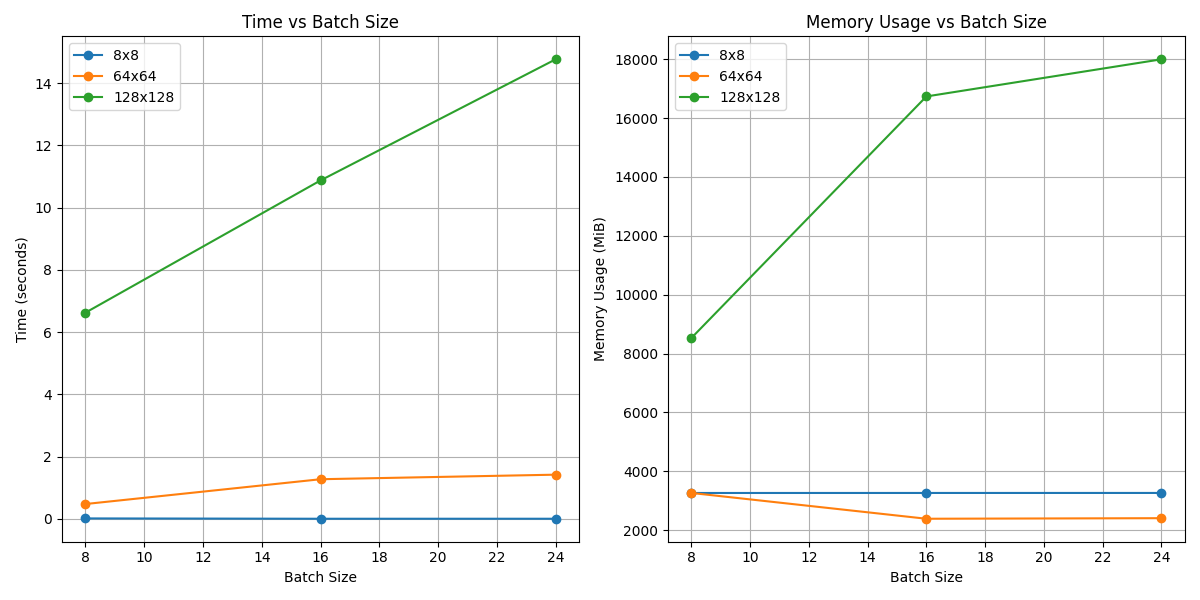
\includegraphics[width=0.8\textwidth]{./figures/score_matching_results}
    \caption{Score Matching Output Graphs}
\end{figure}

    \item \input{03-score-diffusion/02-sliced-score}

    \item \points{3c} \textbf{Denoising Score Matching}

\textbf{Denoising Score Matching (DSM)} enhances Exact Score Matching by addressing the computational challenges associated with directly estimating the trace of 
the Jacobian of the score function. In Exact Score Matching, the trace of the Jacobian matrix can be computationally expensive and 
unstable in high dimensions. DSM avoids this by introducing Gaussian noise to the data and training the model to predict the score of 
the noisy data distribution. This approach indirectly aligns the score function of the model with the true data distribution without 
requiring explicit computation of the Jacobian.

The DSM objective is mathematically defined as:
\begin{align}    
    \mathcal{L}_{\text{denoising}} = \mathbb{E}_{x \sim p_{\text{data}(x)}} \mathbb{E}_{z \sim \mathcal{N}(0, \sigma^2 I)} \Big[ \left\| \mathbf{s}_\theta(x + z) + z/\sigma^2 \right\|^2 \Big],
\end{align}


You are required to implement the following functions in the provided code from \texttt{score\_matching\_utils.py} and \texttt{score\_matching.py} files to make Denoising Score Matching operational:

\begin{itemize}
    \item \texttt{add\_noise}
    \item \texttt{compute\_gaussian\_score}
    \item \texttt{compute\_target\_score}
    \item \texttt{denoising\_score\_matching\_objective}
\end{itemize}

Run the denoising score matching experiment using the following command:
\begin{lstlisting}[language=bash]
    python run_score_matching.py --denoise
\end{lstlisting}

Your implementation should generate the following results:
\begin{figure}[H]
    \centering
    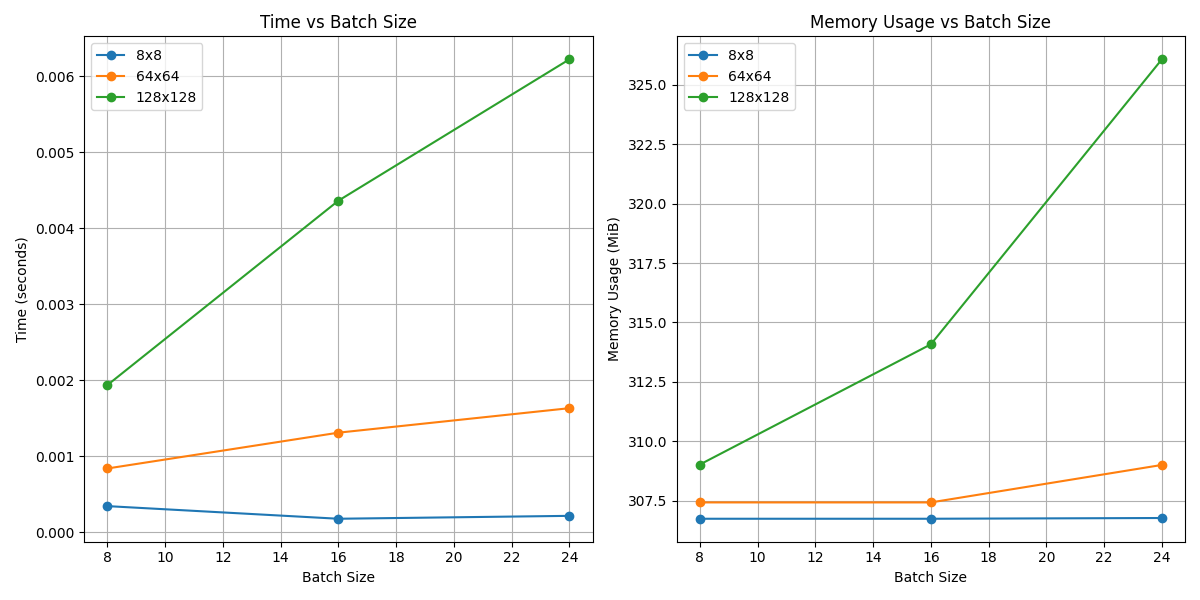
\includegraphics[width=0.8\textwidth]{./figures/denoising_results}
    \caption{Denoising Score Matching Output Graphs}
\end{figure}
\end{enumerate}